\subsection{Performance comparison}
\label{subsec:performanceComparisonDiscussion}

%\textbf{COHEN: How did the program performance compare to its selected standard?} 
%\textbf{Did the program demonstrate good performance?}
%\textbf{Is the programs performance different from predictions?} 
%\textbf{Did you learn what you wanted from the experiments?}

The best route set, having four routes, constructed by the proposed system (CSS), is illustrated in Fig. \vref{fig:bestRouteSet4}. Comparison of the standard ACO implementation and CSS concerning the average produced results is presented in Table \vref{table:performanceComparison_ACOSSOBEST}. The best, worst, and median results along with the standard deviation can be found in Appendix \ref{appendixC}, Table \vref{table:performanceComparison_ACOFull}. 

As one can see in Table \vref{table:performanceComparison_ACOSSOBEST}, CSS performs on average better than the ACO implementation concerning all the proposed performance criteria. Observing Fig. \ref{fig:acovssso}, the ACO implementation performs on average worse than CSS already in the first iteration. One reason for this difference is that the ants in ACO implementations does not possess the ``memory'' attribute. This feature enables the ants to ``remember'' which nodes is already visited in the same route set. Adding this attribute makes the ants favor nodes not visited over nodes already visited, and thus increase the probability of all nodes within the route set being visited at least once. Constraint \vref{itm:criteriaConnectedGraph} specifies that the route network must be connected, and without the added memory, ACO will produce less solutions satisfying this constraint. This again makes ACO produce more route sets that later will be discarded, and thus not evaluated. %The lack of this attribute will thus prevent more (possible better) route sets being explored.  

 \begin{figure}[H]
    \begin{center}
    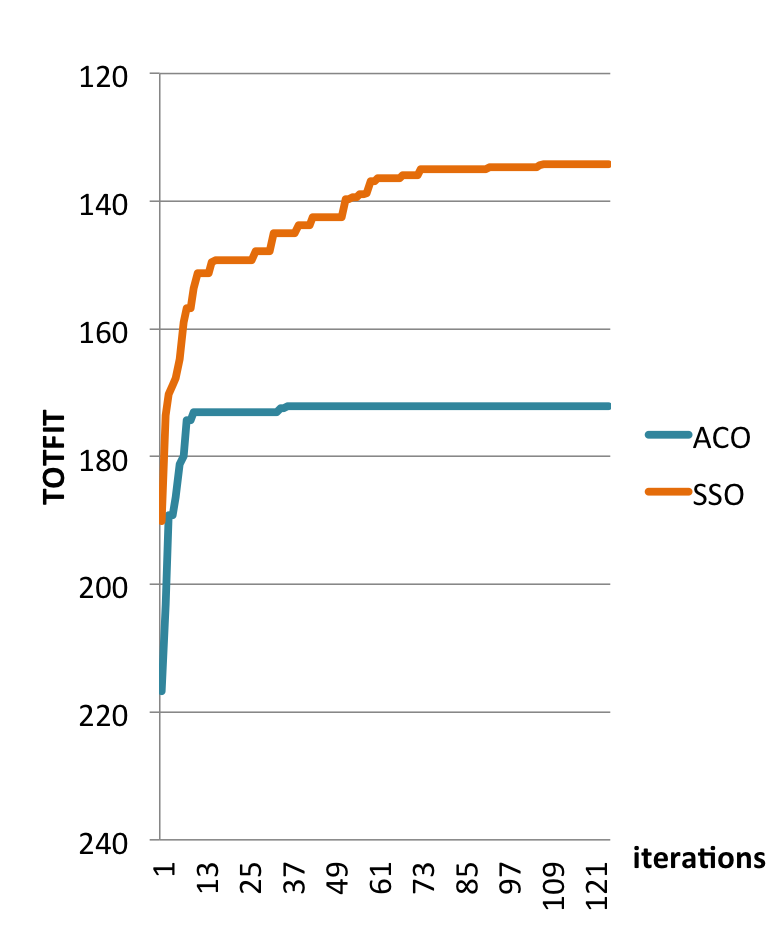
\includegraphics[width=2.5in]{assets/acovsssoNEW.png}
    \end{center}
    \caption{Average TOTFIT value of 10 runs at each iteration for ACO and CSS}
    \label{fig:acovssso} 
\end{figure}

%Kan hente noe info fra setningen over?
Another reason for the difference in performance is because the standard ACO implementation has, as mentioned, a well-known shortcoming of entrapment in local optima. This disadvantage is demonstrated in Fig. \ref{fig:acovssso}. As one can observe, the ACO implementation manage to find good solutions fast. As described in Section \vref{subsec:aco}, the ants will perform a broad search in early iterations, due the lack of distinct pheromone trails. This randomness will decrease over time as the pheromone trails become more defined. Because pheromone evaporate over time, shorter paths will be favored over longer paths simply because shorter paths takes a shorter time. Observing Fig. \ref{fig:acovssso}, after approximately 35 iterations the amount of pheromone on the initial first best routes continue to increase. This will decrease the probability of new ants exploring possible better paths. The evaluation of the route set as a whole is done after each iteration, and this will determine how good the produced route set is. Because of the lack in rewarding the best route sets in the standard ACO implementation, there is no possibility for the ants to communicate information about good solutions.

As one also can see in Fig. \ref{fig:acovssso}, the proposed system manage to get out of this inconvenience, continuing to explore better solutions in the late iterations. Observed in the parameter settings experiment, extracted in Table \vref{table:pm2_inEvaluation}, the additional $CA$ and $AF$ parameters inspired by PSO and BCO, respectively, both improved the average $TOTFIT$ value. 

\begin{table}
    \centering
    %\hspace*{-0.5cm}
    \begin{tabular}{|l|l|l|l|c|}
    \hline
    Parameter & $CA$ & $AF$ & $p_b$ & $AVG(TOTFIT)$ \\
    \hline
    $CA$ & \textbf{0\%} & 10\% & 0.0 & 105.66\\
    ~ & \textbf{25\%} & 10\% & 0.0 & \textbf{103.597}\\
    \hline
    $AF$ (and $p_b$) & 10\% & \textbf{0\%} & \textbf{0.0} & 105.747 \\
    ~ & 10\% & \textbf{5\%} & \textbf{1.3} & \textbf{102.579}\\
    \hline
    \end{tabular}
    \caption {A selection of the average $TOTFIT$ with different parameter values for $CA$ and $AF$}
    \label{table:pm2_inEvaluation}
\end{table}

The $AF$ attribute is added to the proposed system to reward edges in the best route sets with additional pheromone. This feature was partly inspired by \citet{tripathi09} and \citet{sedighpour14}, who demonstrated that rewarding the best solution found so far improved their proposed solution. Rewarding the best solution may also be seen as the recruitment function in BCO. If an artificial bee in BCO has produced a good route set it can ``recruit'' other nest-mates and thus inform the others that a good route set is found. This process inspired to add the ``following'' feature to the proposed system. After the route sets are evaluated, an amount of the best ants with the best route sets is selected to be followed in the next iteration. The same amount of ants will follow the same routes and thus create the same route set. This will increase the pheromone units on the edges chosen by the best ants from the previous iteration, which further increases the probability of them being selected by other ants. Unlike the methods proposed by \citet{tripathi09} and \citet{sedighpour14} are we rewarding the $n$ best solutions, instead of only the very best. Our system performed best with a relatively small amount of followers, but it also benefited from giving these edges additional pheromone ($p_b$). Rewarding edges in a large amount best route sets will result in over appreciating too many edges, which again will make it challenging to distinguish edges in \textit{good} route sets from edges in the \textit{best} route sets. By allowing some ants to be followers, it enables the ants to communicate good solutions with each other. %We believe this increases the performance of CSS. 

However, when the pheromone values on the best edges so far become too high, the probability of discovering new and possible better paths will decrease. The $CA$ attribute was added to the proposed system to ensure more exploring throughout the iterations. $CA$ denotes the amount of ``crazy ants'', which will explore edges random, regardless of the pheromone values. $CA$ is inspired by how the particles in PSO explore solutions. In PSO, as mentioned in Section \vref{subsec:pso}, a decreasing parameter called the inertia weight balances local and global search. This makes the particles becoming more organized in the late iterations. \citet{kechagiopoulos14} showed that PSO can find promising solutions to the UTRP, and our $CA$ attribute are partially inspired by this. To balance the global search by the ``crazy ants'' in the late iterations, the inertia weight ($IW$) inspired by PSO was added to the proposed system. The amount of ``crazy ants'' will decrease in line with $IW$, which again decreases in line with the number of iterations. Decreasing the inertia weight in PSO may result in low global search ability at the end of the run, and thus the possibly of getting stuck at a local optima. However, in the proposed system, the ``crazy ants'' are not searching towards the best-known solution, and may thus prevent the same disadvantage.

%The PSO algorithm enables exploring in early iterations and becoming more organized in the late iteration.
%The parameter is added to balance the local and global search, preventing the particles from drastically changing directions. However, the best global known solution the particles are drawn against may, similar to ACO, be a (possible) local optimum. This parameter can thus enable the algorithm to break out of a (possible) local optima. 

To determine the solution quality of the proposed system, the system is compared to approaches published in the literature. In Table \vref{table:performanceComparison_4}, the results produced by CSS, having four routes, are compared with route sets published in the literature. As one can observe in Table \vref{table:performanceComparison_4},  $d_{unsat}$ is 0, similar to all other approaches. The theoretical best value of for this criteria is 0, which reflects no passenger have to transfer more than two times. All approaches, except \citep{mandl79, kidwai98, chakroborty02}, perform better concerning the $d_0$, $d_1$ and $d_2$ criteria. However, the route set constructed by CSS produce a better $ATT$ compared to route sets constructed by all other approaches. One reason for this is due to how the $TOTFIT$ value is calculated. The calculation of $TOTFIT$ is, as mentioned in Section \vref{sec:totfit}, the sum of $F1$, $F2$ and $F3$. As described in \vref{sec:f1}, a weight parameter, $\sigma$, is used to control the importance of $F1$, $F2$, and $F3$. In the proposed system, $\sigma$ is sat to favor $F1$, which is directly linked to a low $ATT$. Demonstrated in Fig. \vref{fig:mandlWithTT}, when traveling from Node 7 to Node 14, the system will choose to transfer from Route 4 to Route 3, which has a travel time of 20 minutes including a transfer penalty of 5 minutes. As we can see, there is a direct route between Node 7 and Node 14, but this route has a travel time of 27 minutes. As described in Section \vref{sec:totfit}, the route with shortest overall travel time will be chosen. The $F2$ parameter is concerned whether the proposed system has a high $d_0$, denoting a minimum number of transfers. If $F2$ was favored over $F1$, the route set shown in Fig. \vref{fig:mandlWithTT} would get a worse $TOTFIT$ and thus may not be considered as the best route set. It is worth mentioning that the proposed system will not select $F1$ unconditionally. As seen in the produced results, a high amount of $d_0$ is still an important factor when determining the best route set, but the selection of the best route set will be determined concerning the ratio between the two parameters. As mentioned in the motivation of this thesis, citizens often prefer private transportation because of the decreased travel time when no detours are needed. Then again, another important issue concerning passenger satisfiability, is not needing to change vehicles during a trip. Whether a passenger would travel direct with a larger travel time, versus transferring and thus decrease the travel time, is a matter of preferences. As one can see in all the approaches published in the literature including the proposed system, one will have to choose one at the expense of the other. One can argue back and forth about the importance of each criterion. We believe that in a modern urban city, a minimum travel time is the most important factor travelers. This is because some travelers may desire to get as fast as possible from their origin to their destination. We, therefore, choose to emphasize a short travel time. However, as mentioned, the produced route network also possess a relatively high amount of direct routes, giving many passengers opportunities to choose direct routes if it is desired. 
%In the end, it is up to each individual passenger choosing what is most convenient for them. 

\begin{figure}[H]
    \begin{center}
    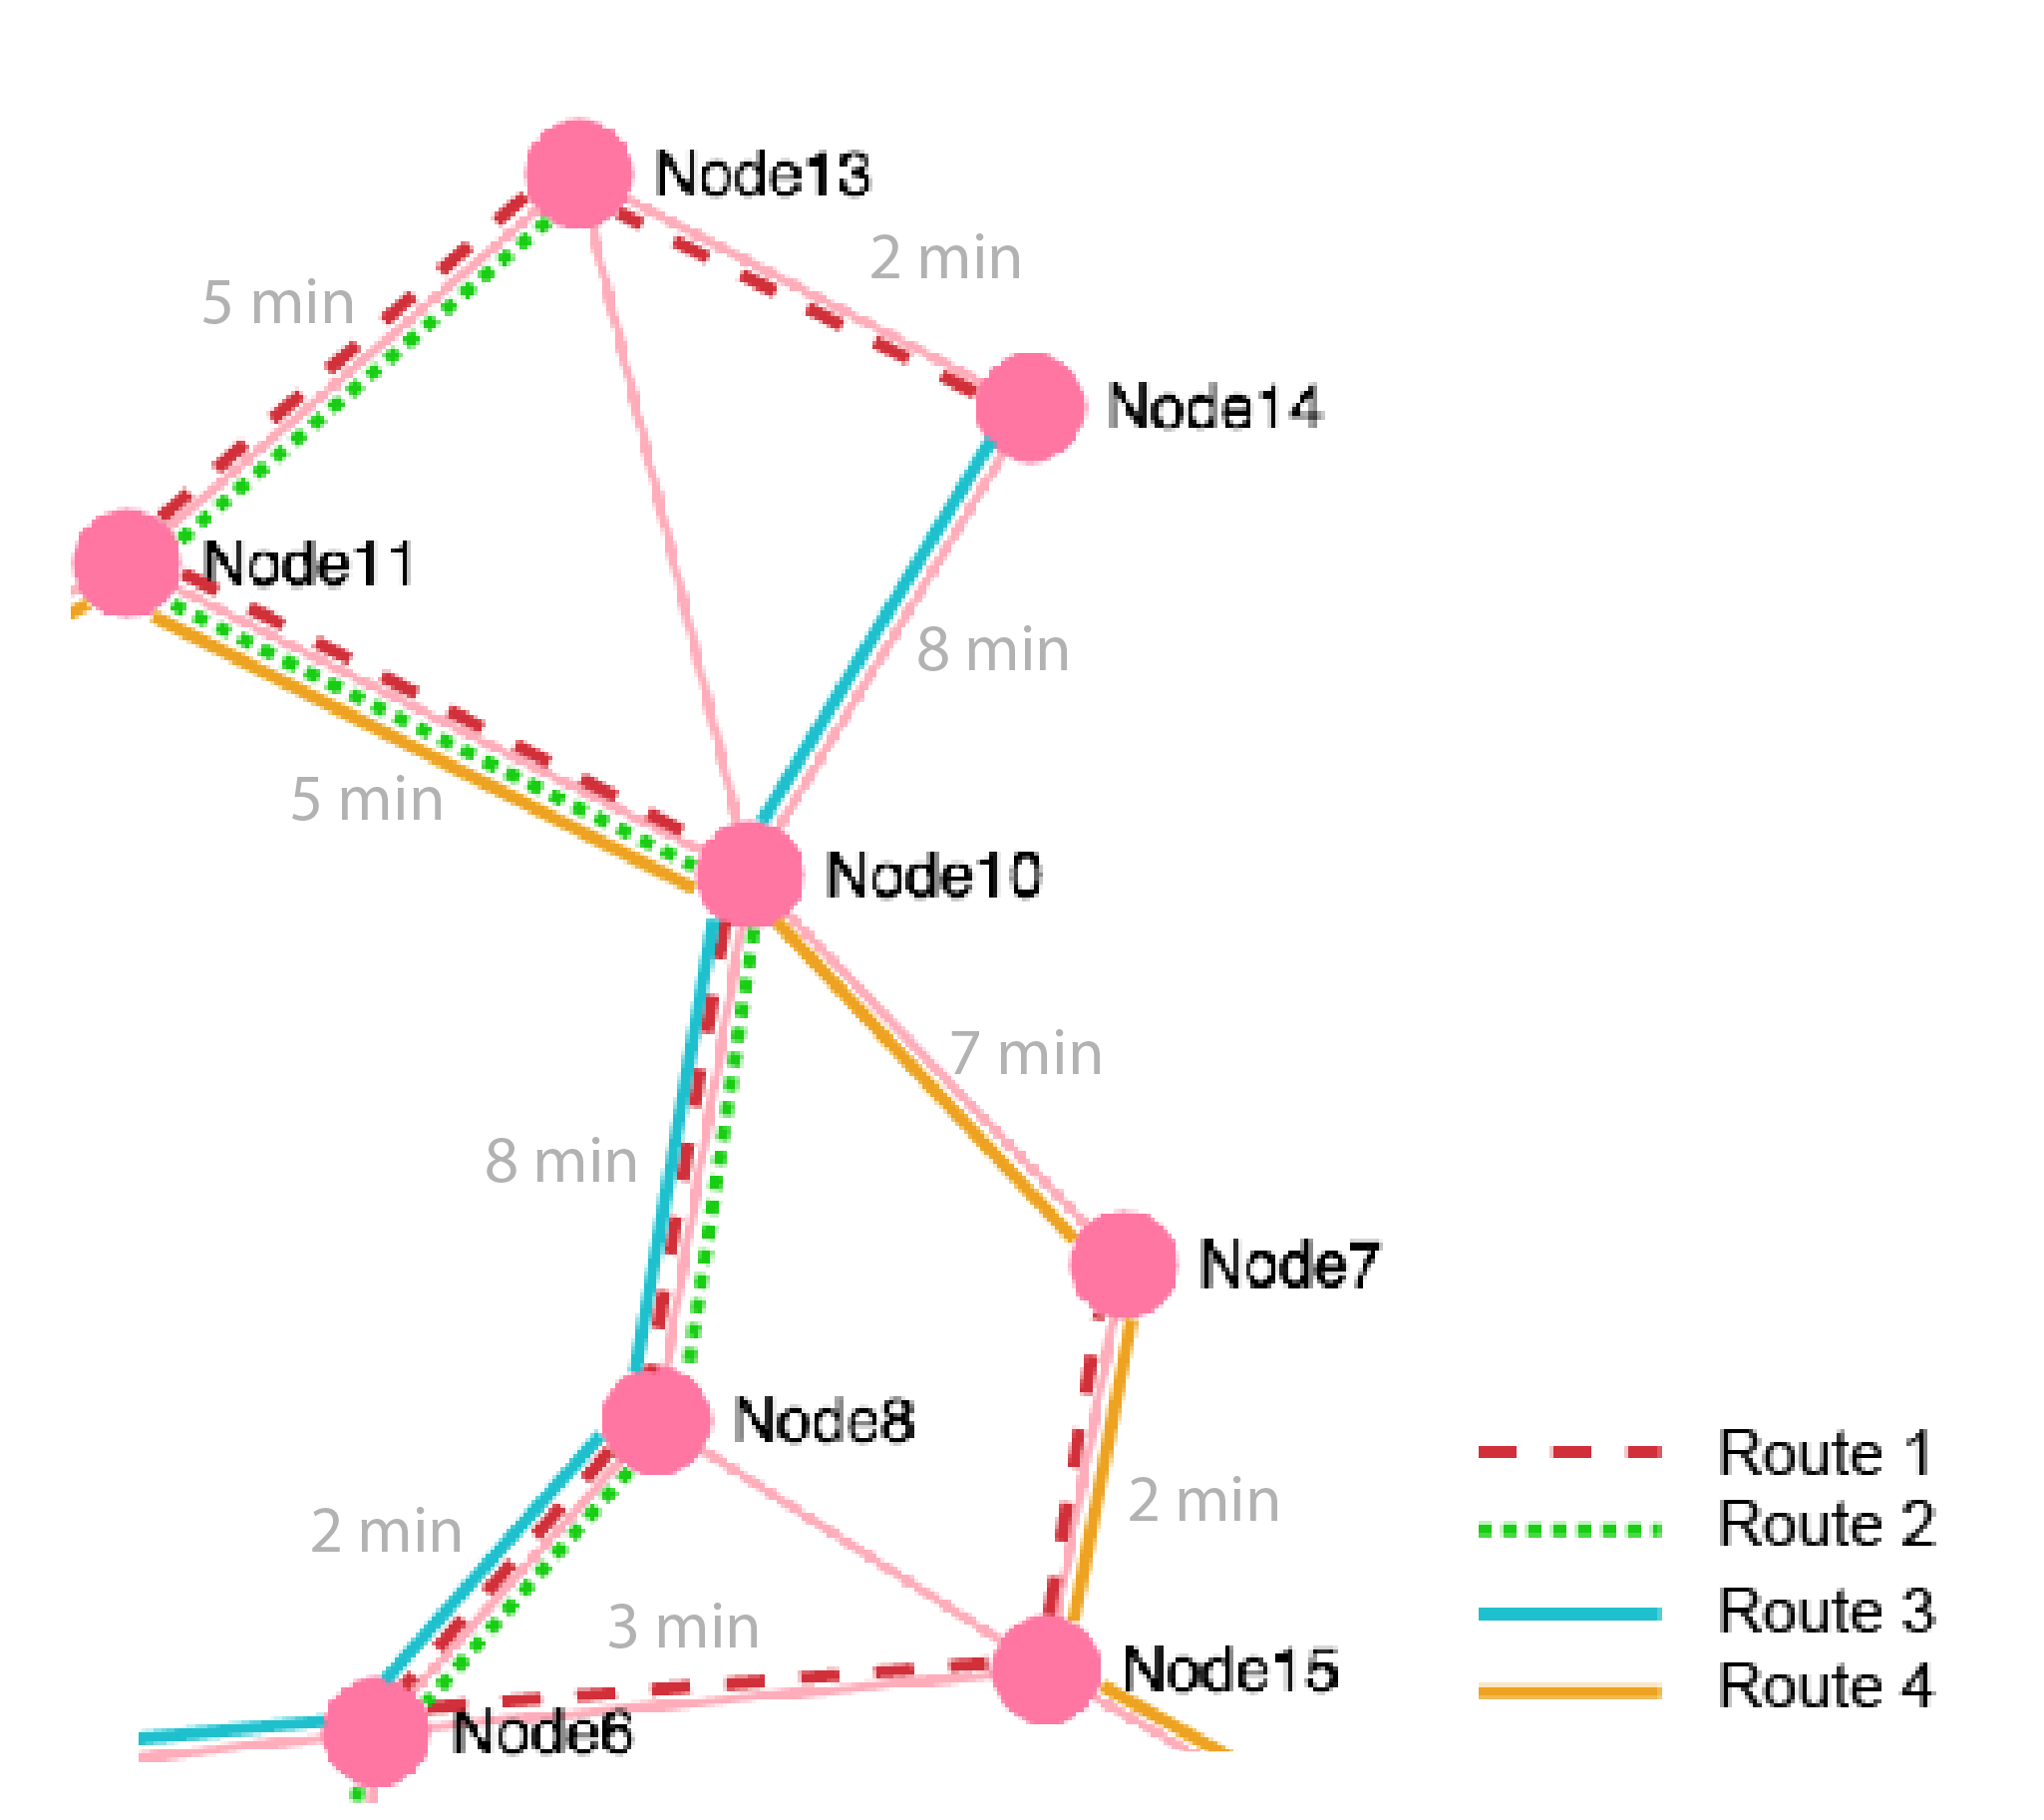
\includegraphics[width=3.5in]{assets/mandl_withTT_utsnitt.png}
    \end{center}
    \caption{A fragment of the best route set, having four route sets, constructed by the proposed algorithm including transfer times in minutes between each node.}
    \label{fig:mandlWithTT} 
\end{figure}

The best route set, having six routes, constructed by the proposed system is presented in Fig. \vref{fig:bestRouteSet6}. The best route set, having seven routes, is presented in Fig. \vref{fig:bestRouteSet7}. The best route set, having eight routes, is presented in Fig. \vref{fig:bestRouteSet8}. The performance comparison for each route set size is found in Table \vref{table:performanceComparison_6}, Table \vref{table:performanceComparison_7}, and Table \vref{table:performanceComparison_8}, respectively. As one can observe, in all route set sizes the proposed system produce a lower $ATT$ than all other approaches, and $d_0$ is below average, whereas $d_{unsat}$ is still 0. As one can observe in Table \vref{table:performanceComparison_routesets}, the amount of direct travelers increase, and the average travel time decrease in line with the number of routes. This corresponds to the growth in performance in all other approaches. The probability of finding direct routes and routes with small travel times will be greater as the number of routes increases. 

 \begin{table}[H]
    \centering
    \begin{tabular}{|l|l|l|l|l|l|}
    \hline
    Route Set & $d_0(\%)$ & $d_1(\%)$ & $d_2(\%)$ & $d_{unsat}(\%)$ & $ATT$ \\
    \hline
    4 & 85.21 & 13.49 & 1.30 & 0.00 & 10.27\\
    6 & 87.17 & 12.0 & 0.82 & 0.01 & 10.11\\
    7 & 88.49 & 10.72 & 0.79 & 0.0 & 10.08\\
    8 & 89.16 & 10.05 & 0.80 & 0.0 & 10.06\\
    \hline
    \end{tabular}
    \caption {Average produced values of the performance criteria for route set sizes four, five, six and seven on Mandl's Network}
    % 50 runs
    \label{table:performanceComparison_routesets}
\end{table}







